%%%%%%%%%%%%%%%%%%%%%%%%%%%%%%%%%%%%%%%%%
% Short Sectioned Assignment
% LaTeX Template
% Version 1.0 (5/5/12)
%
% This template has been downloaded from:
% http://www.LaTeXTemplates.com
%
% Original author:
% Frits Wenneker (http://www.howtotex.com)
%
% License:
% CC BY-NC-SA 3.0 (http://creativecommons.org/licenses/by-nc-sa/3.0/)
%
%%%%%%%%%%%%%%%%%%%%%%%%%%%%%%%%%%%%%%%%%

%----------------------------------------------------------------------------------------
%	PACKAGES AND OTHER DOCUMENT CONFIGURATIONS
%----------------------------------------------------------------------------------------

\documentclass[paper=b4, fontsize=11pt]{scrartcl} % A4 paper and 11pt font size

\usepackage[T1]{fontenc} % Use 8-bit encoding that has 256 glyphs
\usepackage{fourier} % Use the Adobe Utopia font for the document - comment this line to return to the LaTeX default
\usepackage[english]{babel} % English language/hyphenation
\usepackage{amsmath,amsfonts,amsthm} % Math packages

\usepackage{minted} % Allows to put our code :)
\usepackage{graphicx} % Allows to put images :)
\usepackage[usenames, dvipsnames]{color} % Allows to have color :)
\usepackage{tikz} % Used for drawing state machines
\usepackage{pgf} % Used for drawing state machines
\usetikzlibrary{automata, positioning}
\usetikzlibrary{arrows}

\usepackage{sectsty} % Allows customizing section commands
\allsectionsfont{\centering \normalfont\scshape} % Make all sections centered, the default font and small caps

\usepackage{enumitem}

\usepackage{fancyhdr} % Custom headers and footers
\pagestyle{fancyplain} % Makes all pages in the document conform to the custom headers and footers
\fancyhead{} % No page header - if you want one, create it in the same way as the footers below
\fancyfoot[L]{} % Empty left footer
\fancyfoot[C]{} % Empty center footer
\fancyfoot[R]{\thepage} % Page numbering for right footer
\renewcommand{\headrulewidth}{0pt} % Remove header underlines
\renewcommand{\footrulewidth}{0pt} % Remove footer underlines
\setlength{\headheight}{13.6pt} % Customize the height of the header

\numberwithin{equation}{section} % Number equations within sections (i.e. 1.1, 1.2, 2.1, 2.2 instead of 1, 2, 3, 4)
\numberwithin{figure}{section} % Number figures within sections (i.e. 1.1, 1.2, 2.1, 2.2 instead of 1, 2, 3, 4)
\numberwithin{table}{section} % Number tables within sections (i.e. 1.1, 1.2, 2.1, 2.2 instead of 1, 2, 3, 4)

\setlength\parindent{0pt} % Removes all indentation from paragraphs - comment this line for an assignment with lots of text



%----------------------------------------------------------------------------------------
%	TITLE SECTION
%----------------------------------------------------------------------------------------

\newcommand{\horrule}[1]{\rule{\linewidth}{#1}} % Create horizontal rule command with 1 argument of height
\def\changemargin#1#2{\list{}{\rightmargin#2\leftmargin#1}\item[]}
\let\endchangemargin=\endlist

\title{
\normalfont \normalsize
\textit{In The Name of God} \\ \textsc{Computer Engineering Department of Amirkabir University of Technology} \\ [25pt] \horrule{0.5pt} \\[0.4cm] % Thin top horizontal rule
\huge Design Automation Homework - 6 \\ % The assignment title
\horrule{2pt} \\[0.5cm] % Thick bottom horizontal rule
}

\author{Iman Tabrizian (9331032)}

\date{\normalsize\today}

\begin{document}

\maketitle
\section{Question 3}
\begin{itemize}
    \item
        AXI defines the following independent transacation channels:
        \begin{itemize}
            \item
                read address
            \item
                read data
            \item
                write address
            \item
                write data
            \item
                write response

        \end{itemize}

        An address channel carries control information that describes the
        nature of the data to be transferred. The data is transferred between
        master and slave using either:

        \begin{itemize}
            \item
                A write data channel to transfer data from the master to the
                slave. In a write transaction, the slave uses the write response
                channel to signal the completion of the transfer to the master.
            \item
                A read data channel to transfer data from the slave to the
                master.
        \end{itemize}

        Below figures depict how data transfer works in AXI protocol between
        master and slave:
        \begin{center}
            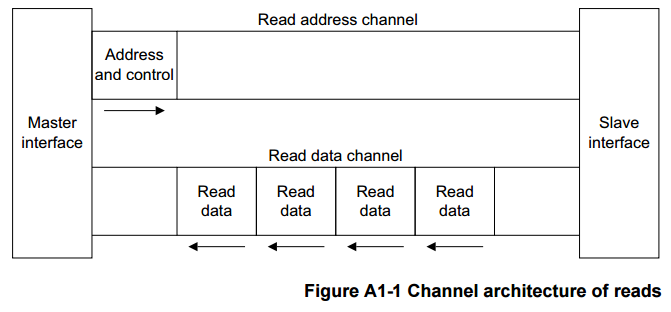
\includegraphics[scale=0.6]{q3/reads.png}
        \end{center}

        \begin{center}
            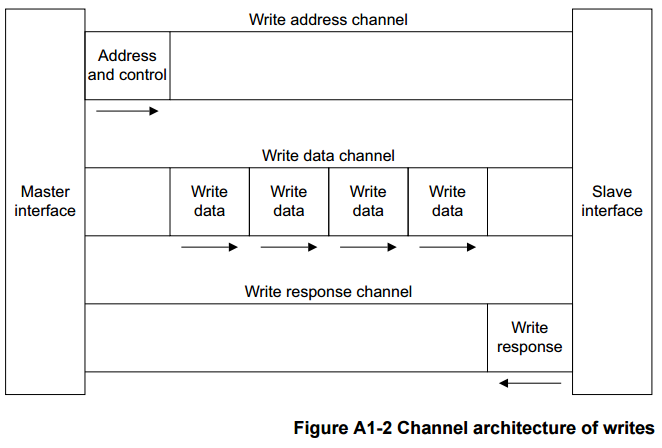
\includegraphics[scale=0.6]{q3/writes.png}
        \end{center}

    \item
        \begin{itemize}
            \item
                \textbf{Stream}: The AXI4-Stream protocol is used for
                applications that typically focus on a data-centric and
                data-flow paradigm where the concept of an address is not
                present or not required. Each AXI4-Stream acts as a single
                unidirectional channel for a handshake data flow.
        \end{itemize}

\end{itemize}




\end{document}
